\documentclass[openany,12pt,a4paper]{report}
\usepackage{subfiles}
\usepackage[numberedsection]{glossaries}
\usepackage[]{graphicx}
\usepackage{float}
\usepackage{multirow}
\graphicspath{{./img/}{./../img/}}
\usepackage{../StileDoc}
\title{Manuale Utente}
\author{}

%Ultima versione documento
\newcommand{\versione}{1.0.0}

% Stile per il glossario
\newglossarystyle{glossaryStyle}{
	\setglossarystyle{altlistgroup}
	\renewcommand*{\glsgroupheading}[1]{
		% Tolgo la numerazione per l'indice
		\setcounter{secnumdepth}{0}
		\section{##1}
		\vspace*{-\baselineskip}
		% Solo per fare un po' di spazio tra la lettera e le voci
		\item\makebox[\linewidth]{\hspace*{2cm}}
	}
}

\glsaddall

\makeglossaries

%Term definitions
\newglossaryentry{Speect}{name=Speect, description={Libreria di Text-To-Speech di riferimento per il progetto DeSpeect}}
\newglossaryentry{GCC}{name=GCC, description={Compilatore C++ di riferimento per il progetto DeSpeect}}
\newglossaryentry{Qt Creator}{name={Qt Creator}, description={Ambiente di sviluppo integrato (IDE) multipiattaforma per creare applicazioni C ++ e QML}}
\newglossaryentry{GitHub}{name=GitHub, description={Servizio di versionamento per progetti software}}
\newglossaryentry{Qt}{name=Qt, description={Libreria multipiattaforma per lo sviluppo di programmi con interfaccia grafica tramite l'uso di widget}}
\newglossaryentry{IDE}{name=IDE, description={un ambiente di sviluppo integrato (in lingua inglese integrated development environment ovvero IDE) è un software che, in fase di programmazione, aiuta i programmatori nello sviluppo del codice sorgente di un programma}}
\newglossaryentry{utterance}{name={Utterance}, description={La più piccola unità del discorso, una parte di esso che inizia e termina con una pausa chiara}}
\newglossaryentry{relation}{name={Relation}, description={Rappresenta una struttura come una parola, sillaba, fonema o anche un obiettivo di durata e gli item sono il contenuto di questa struttura.}}
\newglossaryentry{plug-in}{name={Plug-in}, description={Un programma non autonomo che interagisce con un altro programma per ampliarne o estenderne le funzionalità originarie}}
\newglossaryentry{framework}{name={Framework}, description={Piattaforma che funge da strato intermedio tra un sistema operativo e il software che lo utilizza.}}
\newglossaryentry{issue}{name={Issue}, description={Unità di lavoro per realizzare un miglioramento in un sistema. Un issue potrebbe essere un bug, una funzionalità richiesta, attività, documentazione mancante e così via.}}


\begin{document}
	\makeatletter
	\begin{titlepage}
		\setlength{\headsep}{0pt}  
		\begin{center}
			
\includegraphics[width=0.5\linewidth]{img/logo.png}\\[1em]
			{\huge \bfseries  \@title }\\[10ex]
			\textbf{\Large Informazioni Documento} \\[2em]
			\bgroup
			\def\arraystretch{1.5}
			\begin{tabular}{l|l}
				\textbf{Versione} & \versione{} \\
				\textbf{Data approvazione} & 10 Marzo 2018 \\
				\textbf{Responsabile} & Marco Focchiatti\\
				\textbf{Redattori} &  Manfredi Smaniotto, Marco Focchiatti,\\
				& Cristiano Tessarolo, Giulio Rossetti \\
				\textbf{Verificatori} & Manfredi Smaniotto, Marco Focchiatti \\
				\textbf{Distribuzione} & Prof. Tullio Vardanega \\
				& Prof. Riccardo Cardin \\
				& Mivoq S.R.L. \\
				& Gruppo Graphite \\
				\textbf{Uso} & Esterno \\
				\textbf{Recapito} & graphite.swe@gmail.com \\
			\end{tabular}
			\egroup
		\end{center}
	\end{titlepage}
	\makeatother
	
	\thispagestyle{empty}
	\newpage
	
	%REGISTRO DELLE MODIFICHE
	
	\chapter*{Registro delle modifiche}
	\setlength\LTleft{-22mm}
	\begin{longtable}{|p{20mm}|p{20mm}|p{40mm}|p{30mm}|p{50mm}|}
		\hline
		\textbf{Versione} & \textbf{Data} & \textbf{Autore} & \textbf{Ruolo} & \textbf{Descrizione} \\
		
		\hline 1.0.0 & 2018-04-15 &  & Responsabile & Approvazione \\
		\hline 0.2.0 & 2018-04-15 & - & Verificatore & Verifica da §5 a §8 e appendici \\
		\hline 0.1.4 & 2018-04-14 & - & Amministratore & Stesura appendici \\
		\hline 0.1.3 & 2018-04-13 & - & Amministratore & Stesura §8 \\
		\hline 0.1.2 & 2018-04-12 & - & Progettista & Stesura §7 §3 \\		
		\hline 0.1.1 & 2018-04-12 & - & Progettista & Stesura §5 - §6 \\
		\hline 0.1.0 & 2018-04-11 & - & Verificatore & Verifica da §1 a §4 \\
		\hline 0.0.5 & 2018-04-08 & - & Amministratore & Stesura §4 \\	
		\hline 0.0.4 & 2018-04-08 & - & Amministratore & Stesura §3 \\
		\hline 0.0.3 & 2018-04-07 & - & Amministratore & Stesura §2 \\
		\hline 0.0.2 & 2018-04-06 & - & Amministratore & Stesura §1 \\
		\hline 0.0.1 & 2018-04-05 & - & Amministratore & Creata struttura documento \\
		\hline
		
	\end{longtable}
	
	% INDICE
	\tableofcontents
	
	% INTRODUZIONE
	
	\chapter{Introduzione}
	
	\section{Scopo del documento}
	
	Il documento ha la finalità di illustrare, a coloro che volessero interfacciarsi con l’applicazione
	\textit{"DeSpeect: un'interfaccia grafica per Speect"}, i requisiti necessari per poterlo utilizzare e le modalità di installazione e di utilizzo. 
	Nonostante la versione attuale rappresenti una prima bozza del documento, una volta concluso esso rappresenterà sia una guida che un riferimento completo per l’utilizzo del prodotto da parte di un utente.
	
	\section{Scopo del prodotto}
	
	Lo scopo del progetto è la realizzazione di un’interfaccia grafica per \glossario{Speect}{Speect} [Meraka Institute(2008-2013)], una libreria per la creazione di sistemi di sintesi vocale, che agevoli l’ispezione del suo stato interno durante il funzionamento e la scrittura di test per le sue funzionalità.
	
	\section{Informazioni utili}
	
	La stesura di questo documento assume come utente target del prodotto un programmatore esperto nell'utilizzo di \textit{Speect} e dei linguaggi di programmazione C e C++. \\
	\noindent Per completezza, viene riportato in appendice A un glossario comprensivo di termini tecnici o riguardanti particolari funzionalità di \textit{DeSpeect}. Per identificare i termini presenti nel glossario, la loro prima occorrenza all’interno del documento è riportata in corsivo e marcata con una G al pedice. 
	
	%quando caricheremo su github in una repository apposita il manuale sviluppatore
	\begin{comment}
	\\ \noindent Per i manutentori del prodotto o per chi fosse interessato alla sua integrazione/incremento, può invece consultare il manuale sviluppatore reperibile all'indirizzo: \url{...}
	\end{comment}
	
	\section{Riferimenti informativi}

	\begin{itemize}
		\item \textbf{Documentazione Speect:} \\
		\url{http://speect.sourceforge.net/contents.html};
		\subitem Documentazione ufficiale della libreria di \textit{Text-To-Speech} di riferimento per il progetto.
		
		\item \textbf{Documentazione Qt:} \\
		\url{http://doc.qt.io/};
		\subitem Documentazione ufficiale del \glossario{framework}{framework} utilizzato per lo sviluppo dell'interfaccia grafica.
		
		\item \textit{Documentazione CMAKE:} \\
		\url{https://cmake.org/documentation/}.
		\subitem Documentazione ufficiale del framework utilizzato per la build del prodotto. 
	\end{itemize}

	\chapter{Requisiti di sistema}
	
	L'installazione ed esecuzione del software DeSpeect richiede i seguenti prerequisiti:
	
	\begin{itemize}
		\item Sistema operativo Unix / Unix-like (il software è stato testato solo per piattaforma Ubuntu 16.04 LTS)
		\subitem \url{https://www.ubuntu.com/download/desktop}
		\item CMake (versione minima 2.8)
		\subitem \url{https://cmake.org/download/}
		\item Compilatore ANSI C/ISO C90 \glossario{GCC}{GCC} (versione minima 5.0)
		\subitem \url{https://gcc.gnu.org/install/binaries.html}
		\item \glossario{Qt}{Qt} 5.9.0
		\subitem \url{https://www.qt.io/download}
		\item Git
		\subitem \url{https://git-scm.com/} 
		\item Curl 
		\subitem \url{https://curl.haxx.se/}
		\item Swig 
		\subitem \url{http://www.swig.org/}
		\item libxml2-dev
		\subitem \url{https://packages.debian.org/stretch/libxml2-dev} 
		\item python-dev
		\subitem \url{https://pypi.python.org/pypi/dev/0.4.0}
	\end{itemize}	
	 
	\chapter{Installazione e configurazione} 
	
	DeSpeect è reperibile su \glossario{GitHub}{GitHub} al seguente link:
	\begin{center}
		\url{https://github.com/graphiteSWE/DeSpeect}
	\end{center}
	
	\noindent Una volta soddisfatti i prerequisiti descritti in §2 "Requisiti di sistema" di questo documento, per installare ed eseguire il software è necessario seguire la seguente procedura:
	\begin{enumerate}
		\item Clonare o scaricare la repository sulla propria macchina;
		\item Entrare nella cartella scaricata ed eseguire lo script \verb|build.sh|.
	\end{enumerate}
	Tale procedura installerà la libreria Speect e genererà una build del software nella directory \verb|DeSpeect/build|, nonché avvierà automaticamente un'esecuzione di DeSpeect.
	
	\chapter{Guida all'utilizzo}
	Di seguito è presentata una guida all'utilizzo di DeSpeect.
	I termini evidenziati in \textbf{questo modo} corrispondono a pulsanti presenti all'interno dell'applicazione.
	
	\section{Interfaccia grafica}
	
	\begin{figure}[H]
		
		\centering
		
		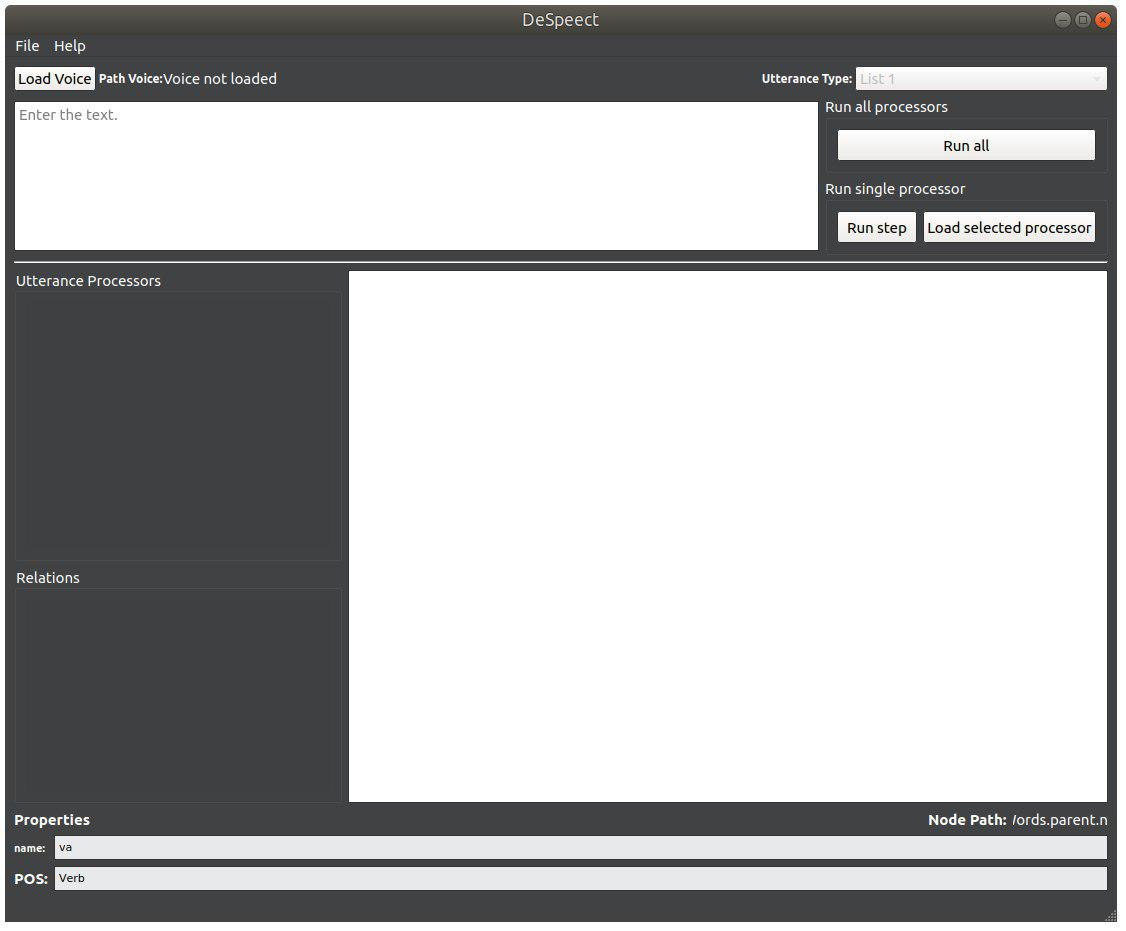
\includegraphics[width=\textwidth]{./img/avvio}
		
		\caption{Interfaccia grafica - Schermata iniziale}
	
	\end{figure}

	All'avvio dell'applicazione viene presentata una schermata come in Figura 1.\\
 	L'interfaccia grafica sarà sempre generalmente composta dalle seguenti componenti:
 	\begin{itemize}
 		\item \textbf{Menù dell'applicazione}: situato nella parte superiore della schermata, dal quale è possibile interagire con \textit{Speect} e con le funzionalità offerte dal sistema (vedi Figura 2);
 		\begin{figure}[H]
 			
 			\centering
 			
 		%	
\includegraphics[width=\textwidth]{./img/menu}
 			
 			\caption{Interfaccia grafica - Menù dell'applicazione}
 			
 		\end{figure}
 	
 		\item \textbf{Pannello di configurazione}: situato sotto il menù, nella parte superiore della schermata, dove è possibile caricare una voice, inserire input testuale, selezionare l'utterance type e avviare l'esecuzione di \textit{Speect} eseguendo singolarmente ogni utterance processors o tutti assieme in una volta (vedi Figura 3);
 		\begin{figure}[H]
 			
 			\centering
 			
 			%	\includegraphics[width=\textwidth]{./img/area}
 			
 			\caption{Interfaccia grafica - Pannello di configurazione}
 			
 		\end{figure}
 	
 		\item \textbf{Pannello degli Utterance Processors}: situato sulla sinistra appena sotto al pannello di configurazione, dove è possibile visualizzare ogni processor e capire quali sono stati eseguiti osservando le caselle relative sulla sinistra (vedi Figura 4);
 		\begin{figure}[H]
 			
 			\centering
 			
 			%	\includegraphics[width=\textwidth]{./img/area}
 			
 			\caption{Interfaccia grafica - Pannello degli Utterance Processors}
 			
 		\end{figure}
 		
 		\item \textbf{Pannello delle Relations}: situato sulla sinistra sotto al pannello degli utterance processors dove è possibile visualizzare le relazioni presenti nel grafo. Qui l'utente può, deselezionando una relazione, togliere i relativi nodi dal grafo (vedi Figura 5);
 		\begin{figure}[H]
 			
 			\centering
 			
 			%	\includegraphics[width=\textwidth]{./img/area}
 			
 			\caption{Interfaccia grafica - Pannello delle Relations}
 			
 		\end{figure}
 	
 		\item \textbf{Area del grafo}: situato sulla destra sotto al pannello di configurazione, dove viene visualizzato il grafo quando viene eseguito \textit{Speect}. I nodi sono selezionabili e si possono spostare (vedi Figura 6);
 		\begin{figure}[H]
 			
 			\centering
 			
 			%	\includegraphics[width=\textwidth]{./img/area}
 			
 			\caption{Interfaccia grafica - Area del grafo}
 			
 		\end{figure}
 	
 		\item \textbf{Proprietà del nodo}: situato nella parte inferiore della schermata, dove vengono visualizzate le informazioni del nodo selezionato (vedi Figura 7);
 		\begin{figure}[H]
 			
 			\centering
 			
 			%	\includegraphics[width=\textwidth]{./img/area}
 			
 			\caption{Interfaccia grafica - Proprietà del nodo}
 			
 		\end{figure}
 		
 	\end{itemize}
	
	\subsection{Menù dell'applicazione}
	Il menù è sempre disponibile in qualunque posizione vi troviate all'interno dell'applicazione e al suo interno è possibile selezionare le seguenti voci:
	\begin{itemize}
		\item File 
			\begin{itemize}
				\item 
			\end{itemize}
		\item Help
			\begin{itemize}
				\item 
			\end{itemize}
	\end{itemize}
	
	\subsection{Visualizzare il manuale utente}
	
	\subsection{Uscire dall'applicazione}
	
	\section{Interagire con la voice}
	
	\subsection{Caricare la voice}
	
	\subsection{Generare l'audio relativo alla voice}
	
	\subsection{Salvare l'audio relativo alla voice}
	
	\section{Stampare il grafo}
	
	\subsection{Importare il grafo}
	
	\subsection{Selezionare gli utterance processors}
	
	\subsection{Visualizzare il grafo}
	
	\subsubsection{Visualizzare il grafo step-by-step}
	
	\subsubsection{Visualizzare l'intero grafo}
	
	\section{Interagire con il grafo}
	
	\subsection{Esportare il grafo generato}
	
	\subsection{Traslare elementi grafici}
	
	\subsubsection{Traslare nodi}
	
	\subsubsection{Traslare archi}
	
	\subsection{Interagire con le relation}
	
	\chapter{Risoluzione dei problemi}
	
	\section{Errori in DeSpeect}
	
	In questa sezione viene fornito un elenco di tutti i possibili errori che si possono riscontrare utilizzando l’applicazione \textit{DeSpeect}:
	\begin{itemize}
		\item \textbf{E01 - ...}:l'utente visualizza un opportuno messaggio di errore nel caso in cui tenti di ...;
	\end{itemize}
	
	\subsection{Struttura dei codici di errore} 
	%Credo vada nelle norme di progetto
	
	\subsection{Log degli errori}
	
	\section{Problemi con il reperimento di Speect}
	
	\section{Segnalazione di bug}
	
	\textit{DeSpeect} potrebbe contenere bug o potrebbe essere desiderabile apportare modifiche e ampliamenti alle sue funzionalità. \\ È possibile segnalare malfunzionamenti o richieste di nuove funzionalità sotto forma di GitHub \glossario{issue}{issue} all’indirizzo:
	\begin{center}
		\url{https://github.com/graphiteSWE/DeSpeect}
	\end{center}
  oppure scrivendo direttamente all'indirizzo e-mail:
  \begin{center}
  	\url{graphite.swe@gmail.com}
  \end{center}
	
	\appendix
	
	\printglossary[style=glossaryStyle, nonumberlist]
	
\end{document}
